% k^2 against the falling square k(k-1), for k=1 to 6.
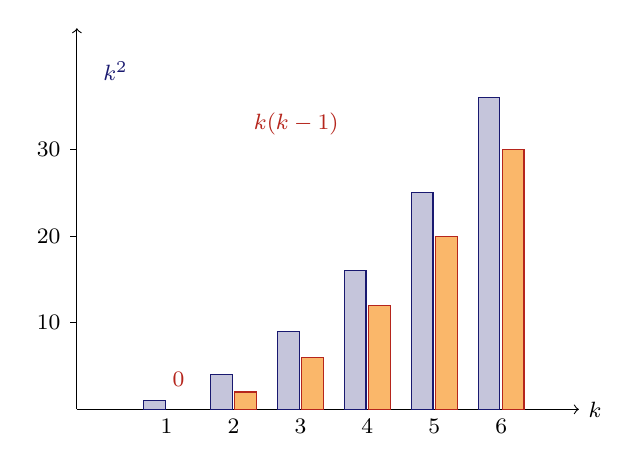
\begin{tikzpicture}[x=0.85cm,y=0.11cm,every node/.style={font=\footnotesize}]
  \draw[->,black] (0,0)--(7.5,0) node[right] {$k$};
  \draw[->,black] (0,0)--(0,44);
  \foreach \k/\h in {1/1,2/4,3/9,4/16,5/25,6/36} {
    \fill[MidnightBlue!25] (\k,0) rectangle (\k+0.32,\h);
    \draw[MidnightBlue] (\k,0) rectangle (\k+0.32,\h);
  }
  \foreach \k/\h in {2/2,3/6,4/12,5/20,6/30} {
    \fill[BurntOrange!55] (\k+0.36,0) rectangle (\k+0.68,\h);
    \draw[BrickRed] (\k+0.36,0) rectangle (\k+0.68,\h);
  }
  \node[BrickRed,anchor=south] at (1.52,1.5) {$0$};
  \foreach \k in {1,2,3,4,5,6} {\node[below] at (\k+0.34,0) {$\k$};}
  \foreach \y in {10,20,30} {\draw[black] (0,\y)--(-0.1,\y) node[left] {$\y$};}
  \node[MidnightBlue,anchor=west] at (0.25,39) {$k^2$};
  \node[BrickRed,anchor=west] at (2.5,33) {$k(k-1)$};
\end{tikzpicture}
